\subsection{Artificial neural networks}
Artificial Neural Networks (ANNs) can be used to approximate functions and are loosely inspired by the structure
of neurons in biological brains.
They have been shown to be able to approximate any continuous function with any desired accuracy \cite{universality_formal,universality_informal}.
A short introduction to ANNs is provided below, see \cite{compint} for more details.

ANNs consist of nodes, also called neurons, connected by directed links (see Figure \ref{feedforward}).
A node is either an input node that receives external input data, an output node which sends out a final value computed
by the network or a hidden node, a node that exists somewhere between the input and output nodes. Each node receives signals, either
as the initial input or as signals from other nodes. Each link is associated with a weight which inhibits or excites the signal
passing over it. The nodes sum up the incoming weighted signals, calculating a net input signal. A function is applied to the net input
signal to generate an output signal (see Figure \ref{neuron}). This function is referred to as an activation function and regulates the strength of the output
signal given the net input signal. The signals are sent through the network until they have reached the final output node or nodes.


\begin{figure}[htb]
    \begin{mdframed}
        \begin{subfigure}[b]{0.5\textwidth}
            \centering
            \resizebox{0.7\textwidth}{!}{\def\layersep{2.5cm}

\begin{tikzpicture}[shorten >=1pt,->,draw=black!50, node distance=\layersep]
    \tikzstyle{every pin edge}=[<-,shorten <=1pt]
    \tikzstyle{neuron}=[circle,fill=black!25,minimum size=17pt,inner sep=0pt]
    \tikzstyle{input neuron}=[neuron, fill=green!50];
    \tikzstyle{output neuron}=[neuron, fill=red!50];
    \tikzstyle{hidden neuron}=[neuron, fill=blue!50];
    \tikzstyle{bias neuron}=[neuron, fill=yellow!50];
    \tikzstyle{annot} = [text width=4em, text centered]

    % Draw the input layer nodes
    \foreach \name / \y in {1,...,3}
    % This is the same as writing \foreach \name / \y in {1/1,2/2,3/3,4/4}
        \node[input neuron, pin=left:Input \y] (I-\name) at (0,-\y) {};

    % Draw the hidden layer nodes
    \foreach \name / \y in {1,...,4}
        \path[yshift=0.5cm]
            node[hidden neuron] (H-\name) at (\layersep,-\y cm) {};

    % Draw the output layer nodes
    \node[output neuron,pin={[pin edge={->}]right:Output 1}, right of=H-2] (O) {};
    \node[output neuron,pin={[pin edge={->}]right:Output 2}, right of=H-3] (1) {};

    % Connect every node in the input layer with every node in the
    % hidden layer.
    \foreach \source in {1,...,3}
        \foreach \dest in {1,...,4}
            \path (I-\source) edge (H-\dest);

    % Connect every node in the hidden layer with the output layer
    \foreach \source in {1,...,4}
        \path (H-\source) edge (O);

    \foreach \source in {1,...,4}
        \path (H-\source) edge (1);

    % Annotate the layers
    \node[annot,above of=H-1, node distance=0.65cm] (hl) {Hidden};
    \node[annot,left of=hl] {Inputs};
    \node[annot,right of=hl] {Outputs};
\end{tikzpicture}}
            \caption{ANN example.}
            \label{feedforward}
        \end{subfigure}
        \begin{subfigure}[b]{0.5\textwidth}
            \centering
            \resizebox{0.9\textwidth}{!}{\def\layersep{2.5cm}
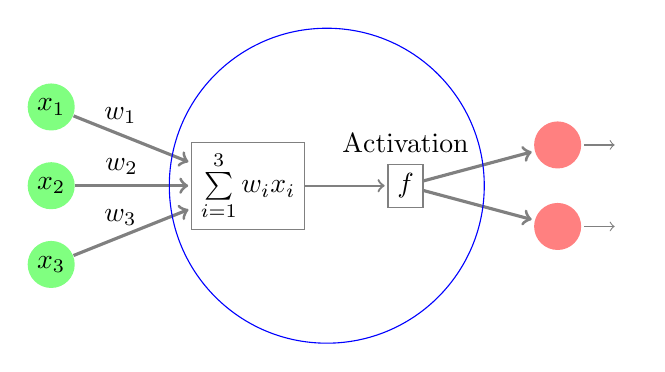
\begin{tikzpicture}[shorten >=1pt,->,draw=black!50, node distance=\layersep]
    \tikzstyle{neuron}=[circle,fill=black!25,minimum size=17pt,inner sep=0pt]
    \tikzstyle{input neuron}=[neuron, fill=green!50];
    \tikzstyle{output neuron}=[neuron, fill=red!50];
    \tikzstyle{every pin edge}=[<-,shorten <=1pt]
    \path
    % Summation
    (0,0)     node[draw] (summation) {$\sum\limits_{i=1}^{3} w_{i}x_{i}$}

    % Input nodes
    +(-2.5,1.0)  node[input neuron]  (input1) {$x_{1}$}
    +(-2.5,0)    node[input neuron]  (input2) {$x_{2}$}
    +(-2.5,-1.0) node[input neuron]  (input3) {$x_{3}$}

    % Activation function
    (2,0)    node[draw] (activation) {$f$} node[above=3mm]{Activation}

    % Output nodes
    +(15:2.0)  node[output neuron, pin={[pin edge={->}]right:}]  (output1) {}
    +(-15:2.0) node[output neuron, pin={[pin edge={->}]right:}]  (output2) {};

    % Link the different parts of the graph
    \draw[->,thick] (summation)--(activation);
    \draw[->,line width=0.4mm] (activation)--(output1) node[pos=.6,above]{};
    \draw[->,line width=0.4mm] (activation)--(output2) node[pos=.6,below]{};
    \draw[->,line width=0.4mm] (input1)--(summation) node[pos=.4,above]{$w_{1}$};
    \draw[->,line width=0.4mm] (input2)--(summation) node[pos=.4,above]{$w_{2}$};
    \draw[->,line width=0.4mm] (input3)--(summation) node[pos=.4,above]{$w_{3}$};
    \draw[blue] (1,0) circle(2);
\end{tikzpicture}}
            \caption{Highlighted path from (a).}
            \label{neuron}
        \end{subfigure}
    \end{mdframed}
    \caption{(a) A feed-forward ANN. (b) Illustration of what happens inside each non-input node of the network; input
                 signals are weighted and summed forming a net input signal to which an activation function is applied.}
\end{figure}

Different algorithms exist to update parameters of the network, such as the weights of the
links, in order to improve the output for different inputs. The process in which the parameters of
the network are optimised is referred to as training. For instance, supervised learning algorithms use input-output
examples to train the network. The input is fed into the network and the output is compared
to the expected output for the example. The difference is used to update the weights in the network in order to decrease
the error. After training with a sufficient number of different examples, the network might generalise and provide
correct outputs for previously unseen examples.
